\documentclass[conference]{IEEEtran}
\IEEEoverridecommandlockouts
% The preceding line is only needed to identify funding in the first footnote. If that is unneeded, please comment it out.
\usepackage{cite}
\usepackage{amsmath,amssymb,amsfonts}
\usepackage{algorithmic}
\usepackage{graphicx}
\usepackage{textcomp}
\usepackage{xcolor}
\def\BibTeX{{\rm B\kern-.05em{\sc i\kern-.025em b}\kern-.08em
    T\kern-.1667em\lower.7ex\hbox{E}\kern-.125emX}}
\begin{document}

\title{Computação de diagnósticos em paralelo\\
}

\author{\IEEEauthorblockN{Gustavo Henrique Jasper}
\IEEEauthorblockA{\textit{Pós-Graduação em Ciência da Computação} \\
\textit{Universidade Federal de Santa Catarina}\\
Florianópolis, Brasil \\
gustavohj6@gmail.com}
}

\maketitle

\begin{abstract}
A identificação de diagnósticos é um problema computacionalmente difícil e está sujeita à demandas por menores tempos de execução. Este trabalho explora alternativas de otimização baseadas em paralelização de busca de diagnósticos.
\end{abstract}

\begin{IEEEkeywords}
Restrições, conflitos, diagnósticos, computação paralela.
\end{IEEEkeywords}

\section{Introdução}

Em aplicações baseadas em resolução de restrições, com frequência ocorrem cenários em que explicações sobre o comportamento da resolução se fazem necessárias. Isso é útil em particular na ocorrência de conflitos.

Configuradores de produto apresentam opções à um usuário baseado em um conjunto de restrições preparado por especialistas. Ao utlizar um configurador de produto, pode estar disponível ao usuário fazer escolhas que conflitam entre si. Também é possível que o especialista responsável por administrar as restrições do produto inicie uma atualização da base de restrições introduzindo uma mudança que não está em acordo com o modelo usado até então.

A figura 1 ilustra um modelo de configurador de produto de um robô de faxina. No modelo é possível identificar características do produto que ficam disponíveis para escolha do usuário. Também é possível idenfiticar restrições entre os valores das caraterísticas.

\begin{figure}[htbp]
\centerline{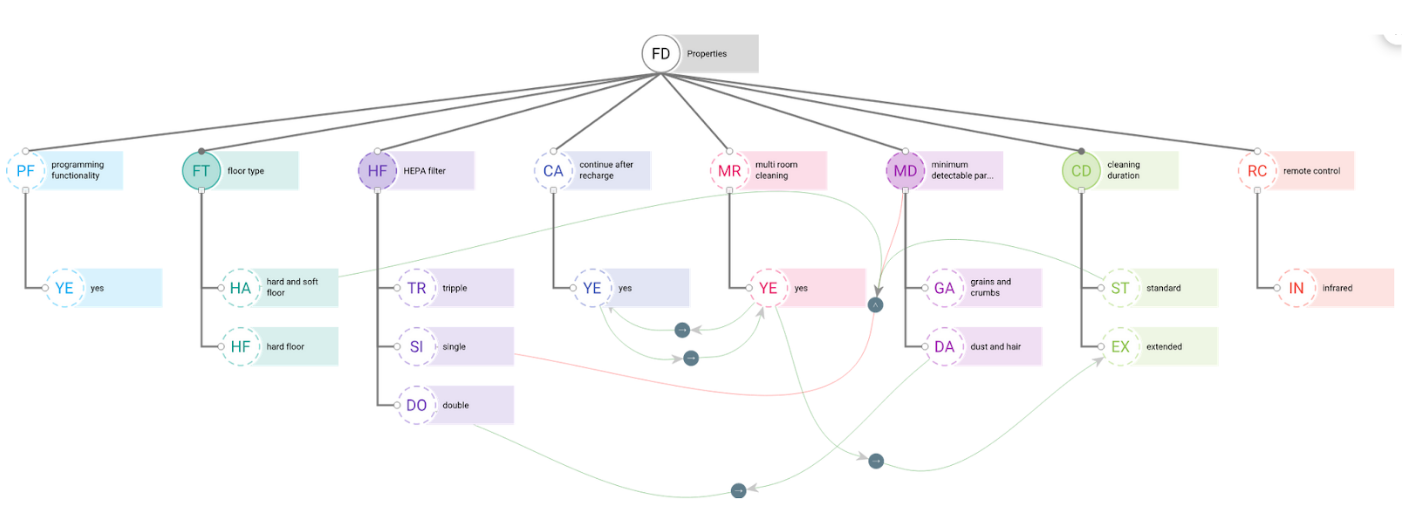
\includegraphics[width=0.7\columnwidth]{model.png}}
\caption{Modelo configurável de um robô de faxina} 
\label{fig}
\end{figure}


Nesse contexto, vem sendo desenvolvidos algorítmos que identificam quais restrições (ou decisões) fazem parte dos conflitos. Uma vez que é possível que mais de um conflito esteja presente em uma certa situação do modelo, outro conjunto de algorítmos vem sendo desenvolvidos para identificar soluções. Essas duas famílias de algorítmos são chamadas de identificadores de conflitos e identificadores de diagnósticos, respectivamente.

A resolução de restrições é um problema NP-Completo. Identificadores de conflito ou diagnóstico são baseados em alguma estratégia de busca em árvore executando a resolução multiplas vezes. É frequente a necessidade de otimização dessas soluções para atender demandas por menores tempos de resposta.

Esse trabalho propõe-se a explorar alternativas de otimização de idenficadores de conflito e diagnóstico por meio de estratégias de computação paralela. 

\section{Trabalhos relacionados}

É possível encontrar trabalhos de otimização de idenficadores de conflito e diagnóstico com computação paralela em publicações envolvendo otimização de configuradores de produto. 

Em [1] é proposto um algorítmo alternativo para a identificação de conflitos baseado em técnicas de de lookahead, onde caminhos alternativos na busca por conflitos são executados paralelamente de forma antecipada. Na medida em que são executados passam a compor uma lookup-table de resultados que é aproveitada pela busca principal.

Em [2] diversas estratégias de paralelização em ambas as etapas (conflitos e diagnósticos) são exploradas. 

\section{Problema abordado}

A computação de diagnósticos ocorre em três camadas, como ilustrado na figura 2.


\begin{figure}[htbp]
\centerline{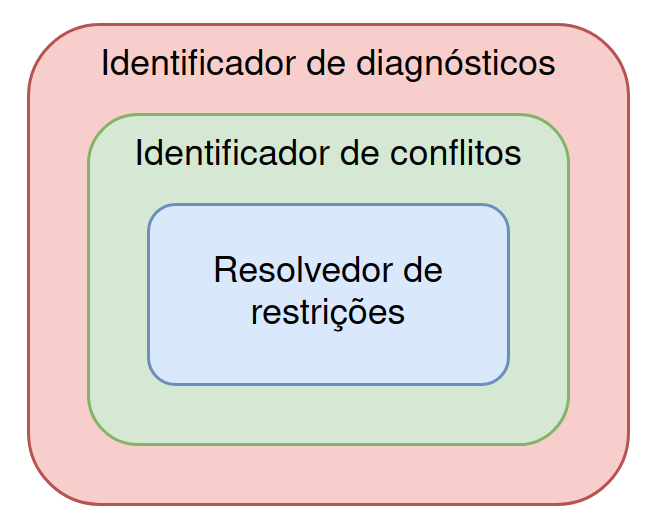
\includegraphics[width=0.7\columnwidth]{layers.png}}
\caption{Camadas da identificação de diagnósticos} 
\label{fig}
\end{figure}

O primeiro nível é um resolvedor de restrições. Para o objetivo de encontrar diagnósticos esse resolvedor pode ter multiplas implementações, tipicamente se trata de uma biblioteca baseada em CSP, SAT, ou equivalente.

O segundo nível é o identificador de conflitos. Trata-se se uma algorítmo de busca em árvore com estratégia de divisão em conquista. A figura 3 descreve o algorítmo desta etapa.

\begin{figure}[htbp]
\centerline{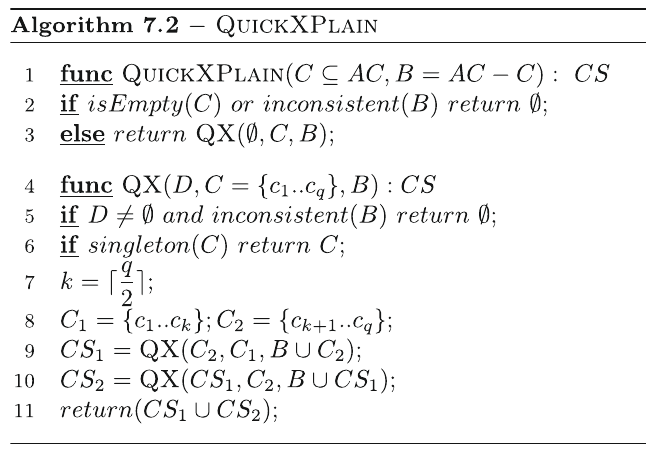
\includegraphics[width=0.7\columnwidth]{qx.png}}
\caption{Algorítmo identificador de conflitos} 
\label{fig}
\end{figure}

O terceiro nível é o idenficador de diagnósticos. Trata-se de um algorítmo de busca em largura. Caminhos nessa busca representam alternativas de diagnóstico. Novos caminhos são identificados a partir da permutação de opções do caminho percorrido até então.

\section{Paralelização do algorítmo}

Em primeira análise foi necessário definir qual etapa teria maior relevância para um trabalho de otimização. As principais alternativas são: A: paralelizar a própria resolução de restrições, B: paralelizar a identificação de conflitos e C: paralelizar a identificação de diagnósticos. 

A estratégia de paralelização da resolução de restrições não é recomendada pelos responsáveis pelos programas resolvedores [3]. Justamente por darem preferência à estratégias de paralelização de busca em um nível superior.

A estratégia de paralelização da identificação de conflitos se mostrou viável, porém só trás ganhos significativos quando baseada em implementações avançadas que se aproveitam de lookaheads [1], ou equivalentes. 

Baseado na análise feita em [2], fica identificado que a melhor candidata à um trabalho de otimização é a etapa de identificação de diagnósticos.

Com essa escolha, tomando como uma implementação sequencial do algorítmo de idenficiação de diagnósticos foi implementada uma alteração no seu loop principal. A implementação de referência utiliza uma estrutura de dados de fila para manter a lista de soluções de condidatas pendentes de processamento. 

A implementação desenvolvida no presente trabalho aproveita-se  dessa fila para processar todos os items pendentes em uma certa iteração do algorítmo ao mesmo tempo. Dessa maneira a progressão da busca acontece de tal maneira que um nível inteiro da busca em largura é processado de forma concorrente. A figura 4 ilustra esse procedimento.

\begin{figure}[htbp]
\centerline{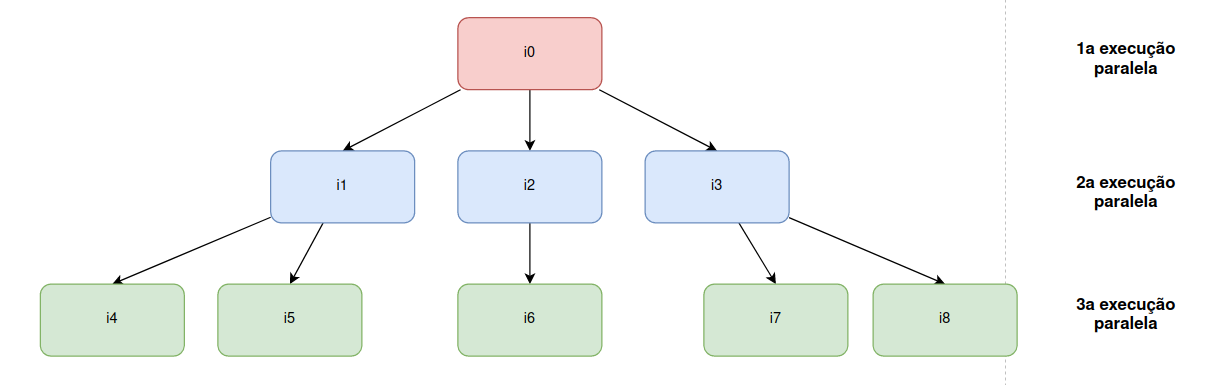
\includegraphics[width=0.7\columnwidth]{runtime.png}}
\caption{Cada nível da busca é uma execução paralela de tasks} 
\label{fig}
\end{figure}

Para implementação dessa estratégia foi usada a técnica de separação de tasks de processamento com retorno do tipo future. Todos os itens na fila são vinculados à uma task assíncrona com retorno future. Na sequência, os futures tem seu valor requisitado e a implementação padrão presente na linguagem se encarrega de realizar a sincronização necessária para continuar o programa quando a respectivas tasks forem concluídas. 

\section{Ambiente experimental}

Uma instância de problema de coloração de mapa foi usada como modelo para testar as implementações. O problema contém 50 variáveis e 150 restrições. Diferentes combinações de restrições adicionais foram introduzidas para gerar conflitos. Na maior configuração haviam em torno de 1500 alternativas de solução para os conflitos. 

Os testes foram realizados em um computador pessoal com 4 núcleos (mais 4 virtualizados).

\section{Resultados}

A figura 5 resume os resultados encontrados nas simulações. Os tempos são informados em milisegundos. Foram computados os tempos de execução da implementação sequencial e paralela, para diferentes cardinalidades de conflitos (3 à 6).

\begin{figure}[htbp]
\centerline{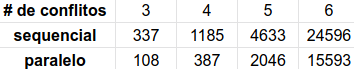
\includegraphics[width=0.7\columnwidth]{result_table.png}}
\caption{Resultados} 
\label{fig}
\end{figure}

É possível observar que houve ganho de desempenho em todas as configurações. Também observa-se que há cardinalidades em que o ganho é mais significativo.

\section{Conclusões}

Identifica-se que há benefício na otimização da busca por soluções de conflito baseada em paralelização da identificação de diagnósticos. Destaca-se que há diversas caminhos não explorados nessa linha, como customização avançada das API de execução paralela, hardware dedicado para execução paralela (em alternativa ao computador pessoal).

\begin{thebibliography}{00}
\bibitem{b1} C. V. Silva, A. Felfernig, J. Galindo, M. Atas, and D. Benavides, “A Parallelized Variant of Junker’s QuickXPlain Algorithm,” in Foundations of Intelligent Systems, vol. 12117, D. Helic, G. Leitner, M. Stettinger, A. Felfernig, and Z. W. Raś, Eds. Cham: Springer International Publishing, 2020, pp. 457–468.

\bibitem{b2} Y. Hamadi and L. Sais, Eds., Handbook of Parallel Constraint Reasoning. Cham: Springer International Publishing, 2018. doi: 10.1007/978-3-319-63516-3.

\bibitem{b3} https://choco-solver.org/docs/
\end{thebibliography}
\vspace{12pt}
\end{document}

